\documentclass[11pt,a4paper]{article}

\usepackage[utf8]{inputenc}
\usepackage{t1enc}
\usepackage[english,magyar]{babel}
\selectlanguage{magyar}
\usepackage{indentfirst}
\frenchspacing
\usepackage{fourier}
\usepackage{graphicx}
\usepackage{makeidx}
\makeindex
\usepackage{url}
\urlstyle{sf}
\usepackage[pdftex,%
    pdfauthor={Barna Gábor},%
    pdftitle={Szoftlab HF specifikáció},%
    pdfsubject={Szoftlab HF specifikáció},%
    plainpages=false]{hyperref}

\author{Barna Gábor}
\title{Szoftlab HF specifikáció}
\begin{document}

\maketitle
%\tableofcontents
%\newpage

\section{Eredeti feladatkiírás}
\begin{quote},,Készítsen GENERIKUS rendezett 3 szintű fésűs listát!

Valósítsa meg az összes értelmes műveletet operátor átdefiniálással
(overload),
de nem kell ragaszkodni mindenáron az operátorok átdefiniálásához!
Amennyiben lehetséges használjon iterátort!

Specifikáljon egy egyszerű tesztfeladatot, amiben fel tudja használni 
az elkészített adatszerkezetet! A tesztprogramot külön modulként
fordított 
programmal oldja meg!
A programmal mutassa be a generikus szerkezet használatát több
egyszerű adathalmazon, amit fájlból olvas be!
A megoldáshoz NE használjon STL tárolót vagy algoritmust!\\
\newline
A tesztprogramot úgy specifikálja, hogy az parancssoros batch
alkalmazásként (is)
működjön, azaz a szabványos bemenetről olvasson, és a szabványos
kimenetre, 
és/vagy a hibakimenetre írjon!
Amennyiben a feladat teszteléséhez fájlból, vagy fájlokból kell input
adatot 
olvasnia, úgy a fájl neve *.dat alakú legyen!
''
\end{quote}

\section{Pontosított feladatspecifikáció}
A generikus fésűs listához C++ sablonokat fogok használni.
A következő operátorok legyenek túlterhelve:
\begin{itemize}
\item \emph{operator+=} - egy új elemet hozzáad a listához
\item \emph{operator-=} - egy adott elemet kikeres és töröl a listából
\item \emph{operator==} - két lista egyenlő
\item \emph{operator!=} - két lista nem egyenlő
\end{itemize}

\newpage
A 3 szintű fésűs listát az alábbi ábra reprezentálja:\\
\newline
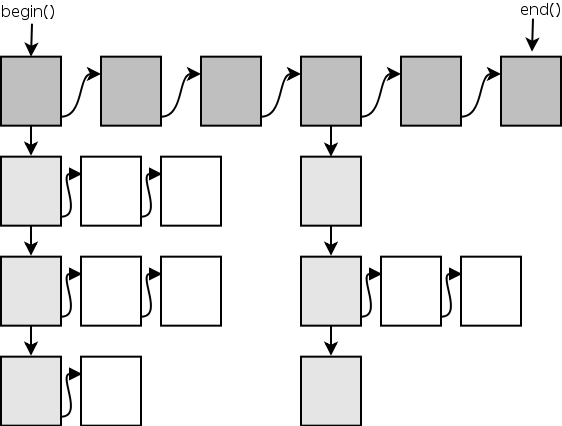
\includegraphics[scale=0.6]{data_structure.png}
\\
\newline
A tároló bejárásához iterátort fogok használni.\\
\newline
Megvalósítandó funkciók:
\begin{itemize}
\item Elem hozzáadása a listához
\item Elem törlése a listából
\item Egy adott elem megkeresése és mutatójának visszaadása\\
\end{itemize}
Az iterátor függvényei:
\begin{itemize}
\item \emph{begin()} - Első elem mutatójának visszaadása
\item \emph{end()} - Utolsó elem mutatójának visszaadása
\item \emph{next()} - Következő elem mutatójának visszaadása\\
\end{itemize}

A tesztprogram képes lesz szabványos bemenetről és fájlból is olvasni.
Mindkét esetben a formátum a következő:
Egy sor egy elemet reprezentál. A három szintnek megfelelően 3 elem
lehet egy sorban (1, 2 vagy 3).\\
\emph{első szint|második szint|harmadik szint\\}
\emph{első szint|második szint\\}

\end{document}
